\chapter{方案设计}
\label{chap:design}
本章重点介绍底层平台感知的高性能NFV平台实现的系统设计。在系统初始化过程中,将动态性能测试的结果作为运行时参数输入系统,后续算法将以该参数作为算法执行时的参照标准。当系统收到一个服务链的请求后,需要根据当前可用的系统资源余量进行判断是否响应,并将上层抽象的业务需求转化为具体的服务链业务链表,系统的映射模块根据服务链的逻辑链表来映射相应的具体实例。在映射实例的过程中,本设计所基于的平台所使用的是随机映射的策略,而这种策略在实际的运行环境中缺乏对底层资源的感知,本设计通过对底层物理资源建模并针对性的提出基于资源亲和度的映射策略,从而提升资源的利用效率。

\section{基于服务链的分析建模}
在虚拟话环境中为NFV应用分配物理资源这个问题可以进一步地划分为两个子问题:(1)虚拟机到物理机的映射问题 (2)在已创建的虚拟节点上映射和调度虚拟网络功能。第一个问题已经有大量的研究来解决,本文主要针对SFC前提下的网络功能映射和调度问题。进一步的,为了在实际场景中解决此问题,我们需要对该问题的前提做一些约束。本文所解决的问题基于以下的假设:
\begin{enumerate}
	\item 每个虚拟机实例仅运行一种特定的网络功能应用。网络功能与虚拟机存在多种多样的映射关系,其中,一对一的这种映射关系目前成为了主流。随着轻量级虚拟机的出现\cite{martins2014clickos,manco2017my},一台物理机上所能承载的虚拟机数量得到了极大地提升,因此这种单一虚拟机单一网络功能的模式可以实现复杂的NFV应用。
	\item 每个虚拟机应当专注于处理本身运行的NFV负载,并且尽量避免由于其他无关业务所带来的性能开销。因为我们选择了单核虚拟机并绑定了虚拟CPU到特定的物理CPU从而减少多核调度所带来的额外开销以及上下文切换。
	\item 针对每种特定的网络功能,都有类似资源池的运行实例群组来保证资源的可用性和可扩展性。
\end{enumerate}

\subsection{关键建模定义}
\textbf{网络功能域}{ }考虑到云计算场景下,各种资源都聚合以资源池的方式对外提供,在NFV场景下也不例外。我们以$D$来表示某种特定网络功能的资源池,也称为网络功能域。
\textbf{服务链}{ }我们用$S$代表一条被映射到具体网络上的网络功能服务链。$S$由一群有序的虚拟网络功能组成$S = \{f_{a} \to f_{b} \to f_{c}\}$,其中,$f$是从特定的网络功能域中选取的运行实例。网络流量根据服务链的连接顺序,依次通过每一个功能节点。
\textbf{多层级映射}{ }如图 \ref{fig:mapping} 所示,除了从SFC描述的抽象逻辑服务链到实际运行的网络功能域中运行实例的映射关系之外,还存在着潜在的从服务链到物理资源的映射。我们用集合$N = \{1,...,n\}$ 来表示一台物理机上所有的物理节点,集合$M = \{1,...,m\}$表示一台物理机上所有的物理CPU,根据CPU所处的物理节点,可以将$M$进一步的划分为$ \{\{1,..m_{1}\},...,\{m_{n},m\}\}$。当服务链与运行实例绑定后,服务链与底层物力资源的映射也随之建立。由于虚拟化软件栈的存在,上层的服务链对于所绑定的底层硬件信息并不知晓。但是实际情况是,如同\ref{label}章中验证性实验所示,底层资源之间的亲和度关系对于整条服务链的性能影响相当严重,所以提升服务链的底层资源亲和度对提升服务链的整体性能具有重要意义。
\begin{figure}[!htp]
	\label{fig:mapping}
	\centering
	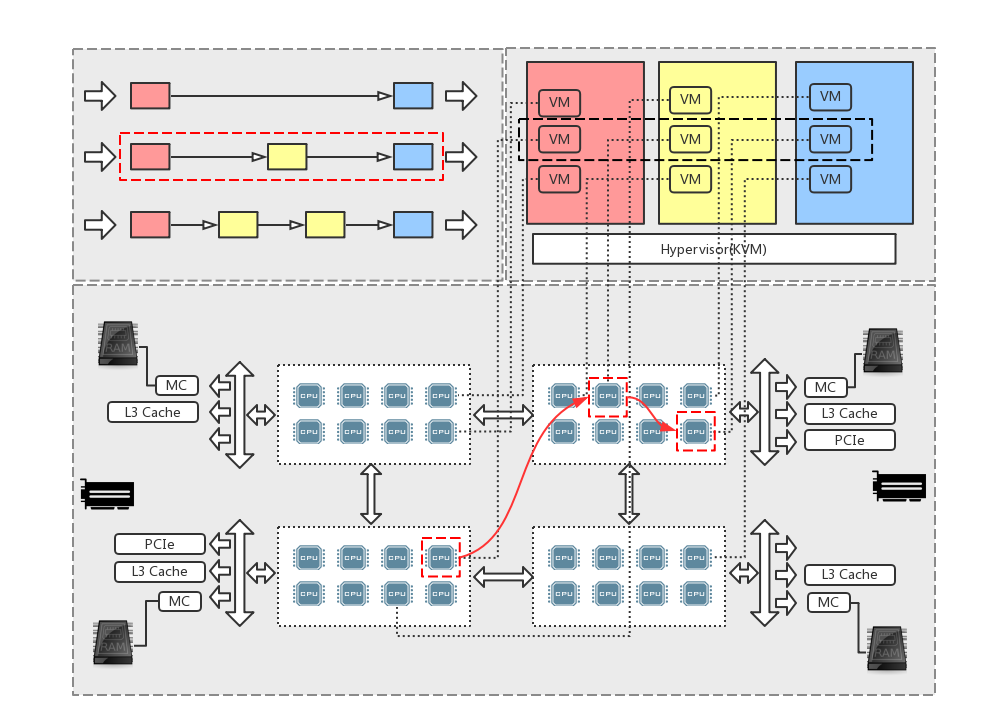
\includegraphics[width=0.8\textwidth]{core.png}
	\bicaption[fig:mapping]{多层级映射关系示意图}{多层级映射关系示意图}{Fig}{Hierarchical Mapping}
\end{figure}

因为NFV中主要的负载是数据流量,所以本文使用衡量网络流量的延迟和带宽参数来衡量NFV的网络性能。我们令 $B_{ij} (i,j \in D, i \neq j)$来表示任意两个运行实例(虚拟机)的的网络通信带宽,令$L_{ij}(i,j \in D ,i \neq j)$ 来表示两者之间通过真实或者虚拟网络通信的网络通信延迟。按照本文的假设,所有的虚拟机仅配置单个物理核,那么显然也存在一个从$f \in D$ 到 $m \in M$的映射。对于服务链上每个虚拟机来说,数据流量将按照串行的顺序沿着数据路径依次通过每个虚拟网络功能节点。为了衡量整个服务链的带宽和延迟,我们需要分析任意两个相连的两个实例之间的带宽和延迟。对于带宽而言,根据串行系统的特性,我们选取整个数据链路上最小带宽作为整条链的带宽值如公式(1)所示。
\begin{equation}
\label{equ:bandwidth}
Bandwidth(S) = \min{(B_{i j } )}  
\end{equation}
对于延迟来说,我们定义了$L(i,j) = L_{i,j} + L_{i} + L_{j}$。其中,$L(i,j)$ 表示数据流量通过以$i$为起点,$j$为终点的服务链的整体延迟,而$L_{i,j}$定义如上文所示表示两个实例的网络传输延迟,$L_{i}$$L_{j}$则分别表示虚拟网络功能处理相关流量而产生的延迟。对于任意一个特定的虚拟网络功能,如果配置了相同的物理资源,则其处理相同网络流量所花费的时间是相同的,也就是说所产生的这部分的延迟是一个固定的值,如公式\ref{equ:latency}所示,则服务链上累计的数据流量处理延迟为与服务链业务相关的常数。但是$L_{ij}$这部分的延迟则由于不同物理资源的组合,存在着很大的变化空间。总的来说,服务链 $S$ 上的传输延迟 $L(i,j)$,主要取决于$L_{ij}$。
\begin{equation}
\Delta Latency(S) = \sum_{i=0,j=i+1}{L_{ij}} 
\end{equation}
\begin{equation}
\label{equ:latency}
\begin{aligned}
Latency(S) & = \sum_{i=0,j=i+1}{L(ij)} \\
& = \sum_{i=0,j=i+1}{L_{ij}}  + C \\
& = \Delta Latency(S) + C  		  \\ 
\end{aligned}
\end{equation}

\subsection{网络服务约束及优化目标}
基于上文中已有的模型,这里我们进一步定义模型中的约束和优化目标,包括服务收益,服务开销,和最终优化目标。


\textbf{服务收益}{ }一个服务链的服务收益 $P$ 可以被定义为通过一定的映射和调度策略下从所使用的物理资源中收获的定量的服务。参照已经由公式 \ref{equ:latency,equ:bandwidth} 定义的带宽和延迟,总体的服务收益可以被视为这两个指标的线性叠加和,其中 $\alpha$ 和 $\beta$为线性表达式的滑动因子,由服务的具体需求来调整。例如,对带宽要求要求的服务则$\alpha$的值较大,而对延迟敏感的应用则有较大的 $\beta$ 值。

\begin{equation}
\label{equ:profit}
P = \alpha*Bandwidth(S) + \beta* Latency(S)
\end{equation}

\textbf{服务开销}{ }我们从所使用的物理资源的角度来定义一条服务链的服务开销。服务链中的运行实体主要是虚拟机,而对于虚拟机而言主要的资源开销为物理CPU,内存,虚拟硬盘和所分配的其他虚拟I/O设备。在本文中,虚拟硬盘和其他虚拟I/O设备与所研究的主题无关故不做考虑。所以,服务开销 $C$ 定义如公式 \ref{equ:cost} 所示。
\begin{equation}
\label{equ:cost}
C = \delta * \sum{CPU} + \theta *\sum{MEM} 
\end{equation}
公式中的 $\alpha$ 和 $\beta$ 分别是做为根据不同需求NFV应用来调节CPU和内存权重的系数。在本文中,结合本文使用的实际应用,我们令 $\delta = 10^{6}$,$\theta = 0.001$ 。从以上定义不难看出,实际的服务开销和服务收益的主要区别在于实际收益中只计算了数据流量在网络功能节点中的处理时间,而实际服务开销则包涵了服务链在传输线路上的传输延迟。

\textbf{优化目标}{ }从一台通用服务器的角度出发,其所拥有的物理资源是有限的,这就意味着所有运行在一台服务器中的服务链的服务开销 $C$ 的和是有上限的。在这样的前提下,为了能够最大化一台服务器的物理资源利用率,我们需要在开销一定的情况下,尽可能地提升服务收益。我们将最终的优化目标设置为 $T$,如公式 \ref{equ:target} 所示,$T$ 为 $P$ 与 $C$ 的累计和之比,即在有限的物理资源的前提下,通过优化的映射策略尽可能的提升服务链的服务收益之和从而达到最大化 $T$ 的最终目标。
\begin{equation}
\label{equ:target}
T = \sum P / \sum C  
\end{equation}

\section{总体设计目标}
数据从一个网络功能节点传输到另一个节点的过程中不可避免的会产生数据处理和传输的延迟,同时物理带宽同样限制着服务理论带宽上限。在标准的工业生产环境中,单个处理器节点中的物理核数量和内存空间也是有限的,同时通用服务器上不平衡的负载分布也会导致剧烈的资源竞争甚至导致意想不到的性能下降。因此,相比于随机的策略,我们需要相对优化的NFV资源映射和调度策略。在本文中,我们的设计主要关注以下是三个目标:
\begin{enumerate}
	\item 物理资源的实际带宽应当满足服务链的最小带宽需求。
	\item 物理资源的数据传输延迟应当小于服务所允许的最大延迟要求。
	\item 物理资源的整体利用率应当得到保证。一个有效的资源映射策略应当可以保证尽可能的使用可用的物理资源,并在相同的物理资源的前提下提升服务的性能。
\end{enumerate}

\section{总体设计思路}
鉴于已有验证性实验的观测结论和以上对此类问题的目标分析和模型建立,本文所设计的系统需要满足实际NFV应用的最小带宽和最大延迟要求,同时在保证服务质量的前提下提升物理资源的整体利用率。

为了实现以上的设计目的,本系统提供了一种基于底层多核运行平台架构感知的虚拟化网络功能的映射方法。在本系统的设计结构中,当NFV平台得到一个服务请求时,会根据服务请求的解析调度虚拟机资源来组织服务链并提供服务。首先NFV管理平台会评估当前服务资源是否满足提供服务的最小需求,即组成服务链的不同功能域中是否有足够的运行实例。当资源充足时,系统开始根据服务链的实际服务数据流转发图来组织服务。在挑选具体服务实例时组成具体SFC时,系统根据预先处理生成的物理资源亲和度矩阵作为调度算法的输入,根据矩阵中每种资源的亲和度大小关系,依照SFC链的连接顺序,使用局部最优的方法搜索构造出最优的服务链与实例的映射关系,最终结果则交由实际映射模块去从虚拟机角度来实现。

从整体架构上分析,实现基于底层多核运行平台的架构感知的虚拟机化网络功能的映射方法,即本文中所设计动态映射系统包括以下关键步骤:

步骤1、对底层平台进行预处理,获得与平台底层运行时相关的信息矩阵。与普通从硬件中读取参数不同,通过动态采样的方法获取平台运行时实时性能参数能更加准确地反映底层平台的架构差异以及所引起的性能差异。首先,动态采用可以实现与操作系统无关,不管多核平台运行的是什么系统,内核是什么版本,不会影响采样程序的运行结果。其次,相比于直接从主板芯片中读取多核架构中不同处理器节点的粗粒度的亲和度信息,动态采样的方法通过动态地运行测试程序,可以获得更加接近实际情况的量化数据。基于这样的数据信息,我们可以更加准确地刻画底层物理资源之间的细粒度的亲和度信息。最终信息被存进格式化的信息矩阵中,作为步骤2的输入。 

步骤2、当一条服务请求到来时,分析该请求所对应的服务链。根据请求所对应服务链的数据流向确定所需要的虚拟网络功能服务点,并依照信息矩阵中的参数大小来确定待映射的具体运行实例,使用基于贪心的方法生成映射决策序列,进入步骤3。

步骤3、根据步骤2生成映射的实例序列,依次检查实例在对应的物理资源节点当前的负载情况,如果某一实例所在节点的负载过高,增加负载会加剧资源竞争导致当前运行实例的性能下降,则返回步骤2将本次的映射序列标记为失效,重新生成新的实例映射序列。检查通过后进入步骤4。

步骤4、根据生成的映射序列,更新默认的随意选取策略,将备选中的实例的Hostname绑定在域名解析服务器中,实现服务链到实际物理资源的映射服务。

步骤5、当服务链服务生命周期结束时,修改域名解析服务器中的记录,重置服务实例状态为待机中,释放实例资源。


\section{模块设计分析}
\subsection{现有的服务链映射策略}
本文的高性能优化系统基于现有的NFV应用平台 Clearwater 来实现。Clearwater的具体架构与模块相关介绍参见\ref{}。在语音和多媒体业务的具体实现中,ClearWater利用云计算资源池化的优势,将各关键网络功能节点以资源池的形式部署在云计算环境中,使用域名解析服务来管理各功能节点之间的连接。默认的服务链实例映射使用随机选取的策略,即根据已有的资源随机选择参与服务组链的运行实例。这样的服务链映射方式随便生成方便管理简单,但是完全忽略了服务链链式服务的数据传输特性,也完全没有考虑底层运行平台的架构差异和资源亲和度信息。同时如果个别处理节点出现负载过高的情况,原有的策略也没有有效的解决方法,甚至有可能加剧某个节点资源竞争,导致服务性能下降的后果。
\subsection{基于底层信息感知的模块设计}
基于对现有平台默认映射策略不足的研究和分析,我们设计了一套底层运行平台感知的高性能NFV系统,该系统架构如图 \ref{fig:system} 所示,想比于原来的服务链映射方式,我们添加了三个模块来实现我们设计目标,即底层信息采样模块 Hardware Sampler,服务链分析模块 Service Analyzer 和动态映射模块 Dynamic Mapper。从图 \ref{fig:system} 中可以看出,我们的系统类似一个中间垫片插入到已有的NFV服务中。上层的业务系统根据具体业务发出服务链服务请求,由管理系统将服务请求下发,服务链需求分析模块收到服务请求后根据具体业务分析出所需服务链,形成组网链表并传递到动态映射模块中。动态映射模块收到服务链表后,根据底层信息采样模块预先生成的信息矩阵生成映射策略,并修改操作域名解析记录来实现组链。
\begin{figure}[!htp]
	\label{fig:system}
	\centering
	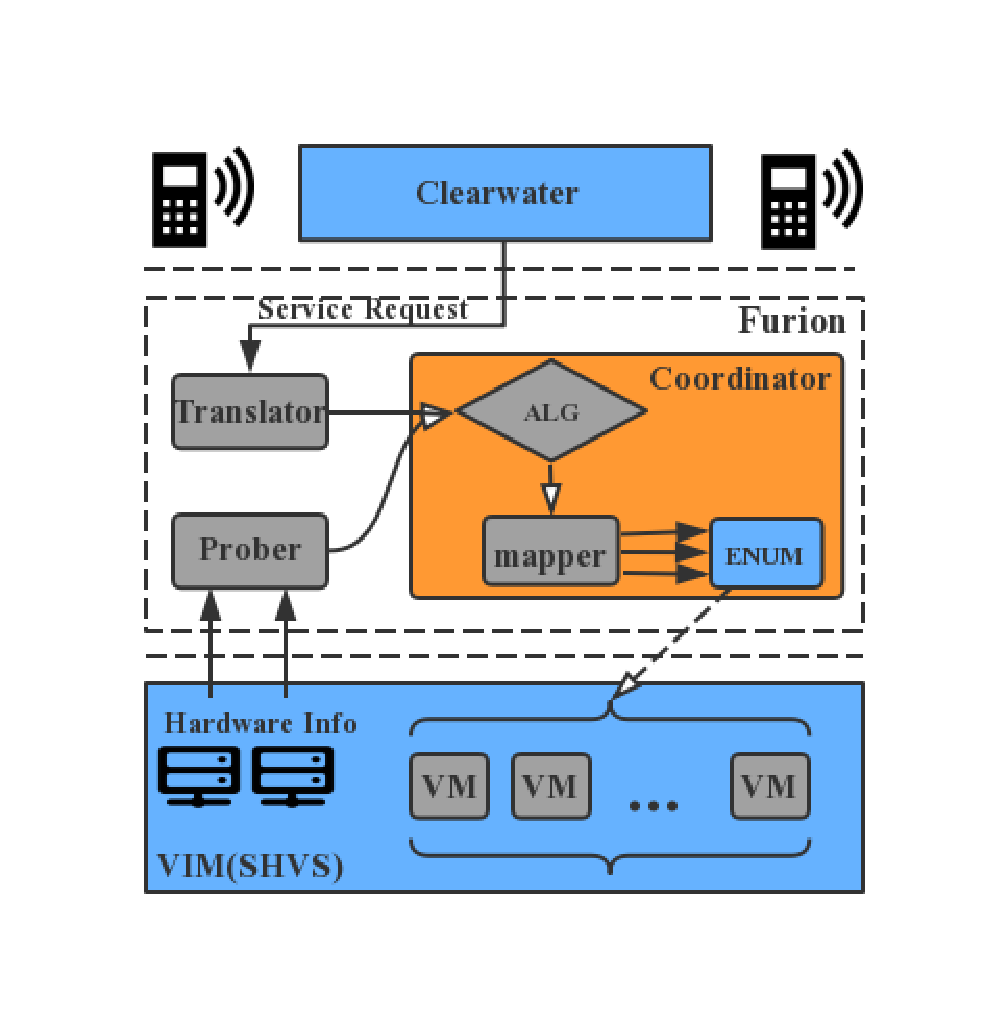
\includegraphics[width=0.7\textwidth]{system.pdf}
	\bicaption[fig:system]{系统架构示意}{系统架构示意图}{Fig}{System Overview}
\end{figure}
\subsubsection{底层信息采样模块}
在系统架构示意图中,底层信息采样模块负责从底层硬件获取运行平台架构信息和运行时各节点细粒度的性能信息。通过预处理采样等手段,该模块将获取的硬件信息以信息矩阵的方式存储下来做系统输入。

\subsubsection{服务链分析模块}
该模块负责在运行时获取并解析上层业务的具体服务请求,将服务请求转化为特定的服务链链表传递给动态映射模块。当特定的服务链链表生成之后,该模块会检查当前运行系统中的资源余量来确定是否响应服务请求。

\subsubsection{动态映射模块}
基于现有的NFV服务平台,我们利用域名解析实现我们的逻辑服务链到实际链路的映射。当动态映射模块收到服务链分析模块传来的特定服务链链表之后,会根据本文提出的基于贪心的算法来生成与逻辑服务链链表相对应的具体实例链表。这里,我们会根据具体实例所在处理节点的实际负载来确定是否重新生成策略。

\section{本章小结}
本章主要介绍了底层平台感知的NFV平台实现方法的设计结构,包括基于服务链的分析建模和本设计的设计目标、设计思路以及详细的模块设计分析。与其他的设计不同,本文从服务链和底层资源的角度出发,进行了相关信息的分析和建模,将物理机的底层资源根据彼此之间的亲和度关系划分为了不同的等价类,并从上层应用的运行实例的角度出发定义了不同物理资源前提下的应用运行所需的成本和随之带来的开销。在所建立模型的基础上,我们提出了设计的所关注的三个目标,并以这些目标作为约束详细阐述了我们的总体设计思路和模块的设计细节。